%////////////////////////////////////////////////
% ToDo:
% 3D: Meshes, Materials, Textures, UV
% Game Engines
% Renderers (Blender)
% URDF
%////////////////////////////////////////////////


\chapter{Theoretical Background}

% //////////////////////////////////////////////////
\section{Object Recognition using Convolutional Neural Networks}
Everyday tasks performed by humans require exact recognition and categorization of objects in order to perform actions like manipulating objects. 
% Beispiele, konkreter
These skills can further be used to deduce an understanding of one's surroundings and effectively grasp the context one acts in. These tasks are easily and for the most part subconsciously performed by humans but prove to be a challenge for software.\
\subsection{General Working Principle}
\acp{CNN} are a type of \acp{ANN} that operate on high-dimensional input data. This includes regular images in raster formats as their pixels are organized in rows and columns and color channels resulting in a three-dimensional input volume. These networks consist of multiple layers: the first layers will prepare the input data for later use (e.g. by performing scaling down the input data).\\
Next, \ac{conv} layers further process the input data. Those have a set of learn-able filters that are the artificial representation of biological neurons and perform convolutions on small chunks of data, that extend through the full depth of the input volume \cite{Schweitzer2017}, along the input data (e.g. by sliding through images row-by-row and column-by-column) where they process local pixel data depending on their implementation and the size of their receptive field. For instance, by performing edge-detection (using e.g. the Prewitt, Roberts or Sobel operators \cite{5557884}), filters may uncover features. Each of these filters will output a two-dimensional activation map that contains their responses at every position of the input data \cite{cs231n}. Stacking these activation maps yields a three-dimensional output volume.\\
The output of \ac{conv} layers is a linear function. In order to solve real-world problem that are non-linear though, non-linear layers are applied to the output of \ac{conv} layers. In simplified terms, those layers map the data from an input volume to a specified, non-linear range of values (e.g. from 0 to 1). There are various non-linear functions that can be used, a popular one is the \ac{ReLU} which maps negative values and keeps positive values. It is simple to implement and does not involve expensive computations.\\ %Drawbacks?
Pooling layers are used to reduce the size of the input data by applying filters to it. There are various methods that can be used, such as the average-pooling that chooses the average value of inputs. By reducing the size of inputs, pooling layers effectively reduce the complexity and number of weights in following layers, hence processing by following layers require less computation time. Chaining layers by using the output of one last layer as an input for another layer allows to detect more complex features as the filters of the other layers would be trained using refined data.\\
Lastly, at end of a \ac{CNN} will be one or more \ac{fc} layers. Those translate an input volume to a set of $n$ values where each value represents one class the network can choose. Each of these values would represent the probability of its class. This translation is done by learning from the input volume which is a stack of activation maps of complex features. Certain combinations of high values in those maps will indicate specific classes like the detection of a long body with multiple wheels on a flat ground may be interpreted as a vehicle.\\
Figure \ref{fig:lenet5} shows the architecture of LeNet5 by LeCun \textit{et al.} from 1998. It should prove to set a pattern for modern \acp{CNN} by utilizing multiple sets of \ac{conv}, non-linearity and pooling layers, forwarding their processed data to multiple layers for classification. One of its successors is AlexNet, designed by Alex Krizhevsky \textit{et al.} in 2010 \cite{NIPS2012_4824} which is still a relevant measure for modern \ac{NN} today \cite{DBLP:journals/corr/CanzianiPC16}.

\begin{center}
\noindent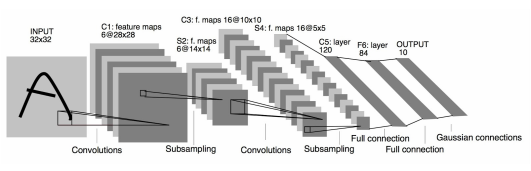
\includegraphics[width=12cm]{tex/img/ch03/LeNet5.png}
\captionof{figure}{Architecture of LeNet5 that set a pattern for modern \acp{CNN} \cite{Lecun98gradient-basedlearning}}
\label{fig:lenet5}
\end{center}

\subsection{Data Augmentation}
In summary it can be stated that \ac{conv} layers are trained to detect features and \ac{fc} layers are trained to detect relations between features that indicate specific classifiers. To achieve this, \acp{CNN} need to be trained with datasets specific to their application that must be of good quality \cite{Schweitzer2017}. Factors contributing to the quality of datasets are the quality of their images (e.g. high resolution, little noise) and labels (e.g. number of classes, general presence of regions associated with labels). However large sets of such data may be hard to come by due to scarce availability (e.g. of datasets for highly specialized applications) or the amount of effort creating those takes. Lastly, they may simple cost a lot of time to produce.\\
\textit{Data Augmentation} promises to solve this problem by altering datasets through application of various operations on them: for instance images can be stretched, mirrored, zoomed and rotated or color filters can be applied to them. As long as these changes are transferred to the labels of images, these altered datasets drastically increase the size of datasets that can be used for training \acp{CNN}. This can also potentially help to make detections more reliable for special cases: for instance, datasets that feature cars would mostly show cars in their surroundings, hence they would rarely be cut off in images. Altering images so they cut off parts of cars like wheels may enable \acp{CNN} to recognize cars without requiring cars to actually have wheels.

\section{3D Graphics}
\subsection{Transforms}
As this chapter is about 3D graphics, this section will handle exclusively 3D transforms. In computer graphics, all locatable objects in 2D or 3D space use transforms to express their location, rotation and scale. Those attributes can be expressed in vectors with three elements each, where each of these elements represents the effect of a transformation for one axis. A complete transformation with a location $l$, rotation $r$ and scale $s$ for an object could be written as:
\begin{center}$l = \begin{pmatrix} 0\\0\\0\end{pmatrix}, r = \begin{pmatrix} 0\\90\\0\end{pmatrix},  s = \begin{pmatrix} 1\\1\\1\end{pmatrix}$\end{center}
This describes an object that is located at the center of the coordinate system, is rotated around the y axis by $90$ degrees and has the default scale of $1$ applied to all axis.
\cite{10.1007/978-1-4471-6290-2}
\subsubsection{Operators}
\paragraph{Translation}
\paragraph{Scaling}
\paragraph{Rotation}


Transformations (world-space, local-space), Projections (screen-space)

\paragraph{Meshes} \textit{Vertices} are data-structures that hold information about points in 3D space (\ref{fig:3d-vertices}). Depending on the application, vertices can hold additional information, e.g. color and reflectance. Vertices can be connected to each other via \textit{edges} (\ref{fig:3d-edges}). \textit{Faces} are planar surfaces defined by a set of usually three (polygon) or four (quad) edges (\ref{fig:3d-face}). Vectors that are perpendicular to faces are called \textit{normals} and are often used in rendering, for instance to calculate light-reflections on surfaces). A \textit{mesh} is an individual set of vertices, edges and faces (\ref{fig:3d-mesh}). 
% Meshes: Warum? Annäherung an die Realität, nur Körper (nur 3D, keine Textur), Uses

\begin{figure}[!htb]
\minipage{0.25\textwidth}
    
\includegraphics[width=\linewidth]{tex/img/ch03/Basics01_Vertices.png}
    \subcaption{Vertices}
    \label{fig:3d-vertices}
\endminipage\hfill
\minipage{0.25\textwidth}
    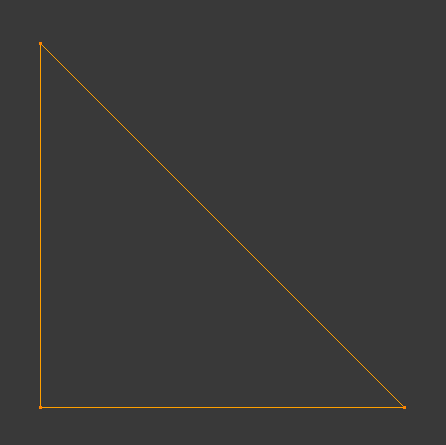
\includegraphics[width=\linewidth]{tex/img/ch03/Basics02_Edges.png}
    \subcaption{Edges}
    \label{fig:3d-edges}
\endminipage\hfill
\minipage{0.25\textwidth}%
    
\includegraphics[width=\linewidth]{tex/img/ch03/Basics03_Faces.png}
    \subcaption{Face}
    \label{fig:3d-face}
\endminipage
\minipage{0.25\textwidth}%
    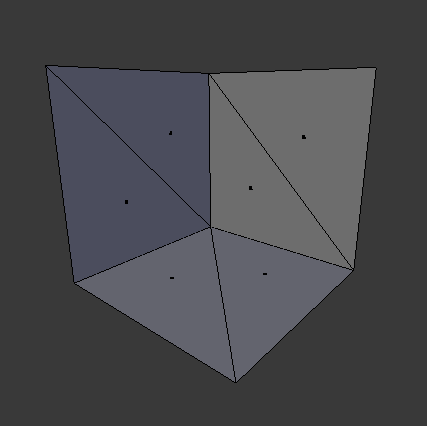
\includegraphics[width=\linewidth]{tex/img/ch03/Basics04_Meshes.png}
    \subcaption{Mesh}
    \label{fig:3d-mesh}
\endminipage
\captionof{figure}{Construction of a mesh}
\end{figure}

\paragraph{Materials} \textit{Textures} are images that are mapped to meshes for various uses. They can be used to encolor a mesh, manipulate its vertices height (\textit{Heightmap})\cite{UnityDocHeightmap} and simulate bumps (\textit{Normalmap}\cite{UnityDocNormalmap}\cite{Cohen:1998:AS:280814.280832}\cite{745285}) and reflections (\textit{Specularmap})\cite{UnityDocSpecularmap}.\\
\textit{UV-maps}.
Mapping textures to meshes requires a \textit{UV-map}

\begin{center}
\noindent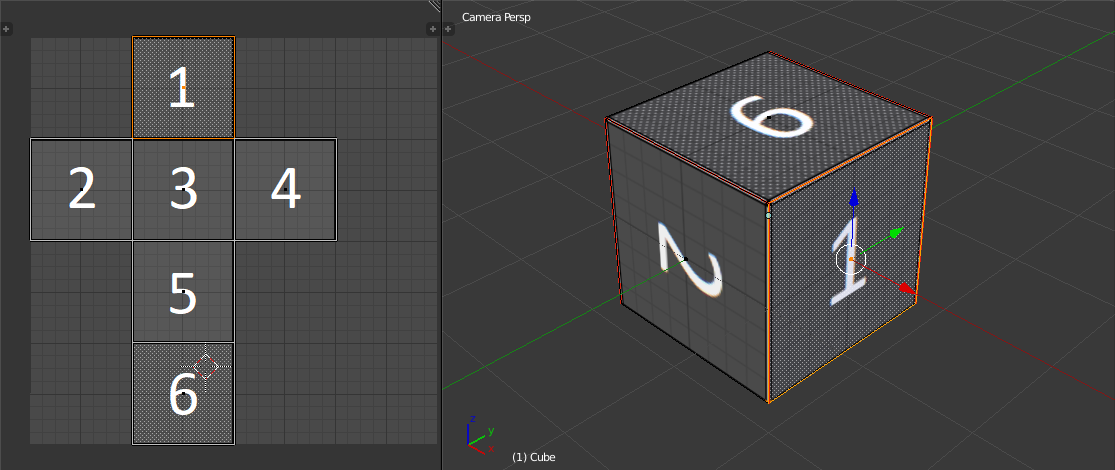
\includegraphics[width=12cm]{tex/img/ch03/CubeUVMapping.png}
\captionof{figure}{UV-map of a cube on top of a texture (l) and the same texture being applied to a cube (r) using the same UV-map where the face showing a "1" is highlighted.}
\label{fig:3d-cube-uv-mapping}
\end{center}

\subsection{Rendering}
Raytracing \cite{Plemenos2010} vs Rasterization [TBD]
Post-Processing: ambient occlusion, anti-aliasing, depth-of-field, high dynamic range, shading [TBD]

%- Definition
   %- Techniques
%- Photorealism (Physics)

\subsection{Blender}
%- Why this one? (free, active development, support, cross-platform)
[TBD]

% //////////////////////////////////////////////////
\section{Game Engines}
Definition, Overview, Concepts (Entity Component System, Asset Bundles) [TBD]
%- Definition
%- Overview
%- Concepts
%- Workflow (!!!)

% //////////////////////////////////////////////////
\section{Unified Robot Description Format}
\ac{URDF}